In any 3D application we are creating a mathematical model to represent the objects within a given scene. Therefore mathematics plays a very large part in many areas of 3D graphics. Three dimensional mathematics makes use of trigonometry, algebra and even statistics, however in the interest of time, I will be mainly focusing on the specific concepts used in 3D vector, quaternion and matrix mathematics. These concepts contribute to the representation of 3D models as well as model transformations such as: translation, rotation and scaling.  

\section{Points and Vectors}

When representing objects we need to keep track of where they are in the virtual world. In a 2 dimensional world this may be represented by two numbers, an X and a Y position. In 3 dimesions we can represent this with X, Y and Z positions. 3D objects are will usually have a point of origin or global position but in most 3D applications, points or vectors make up triangles. One triangle can be said to be a face and multiple faces will make up a 3D object. In this section we will be looking at the use of points and vectors in 3D graphics.

\subsection{Points} 

A point is a position in space of $n$-dimensions. In computer graphics applications we usually deal with \acrshort{2d} or \acrshort{3d} coorinate systems. The most common coorinate system used in computer graphics is cartesian coorindates. Cartesian coordinates of a \acrshort{2d} system can be represented by an ordered pair of perpendicular axes, which can be represented as $(p_x, p_y)$. Similarly a point in \acrshort{3d} space can be represented by an ordered triple of perpendicular axes, represended in the form $(p_x, p_y, p_z)$. This can be represented in figure \ref{3DAxisFigure} below.

\begin{figure}[htbp]
	\raggedright
	{\centering
		\vspace{7px}
		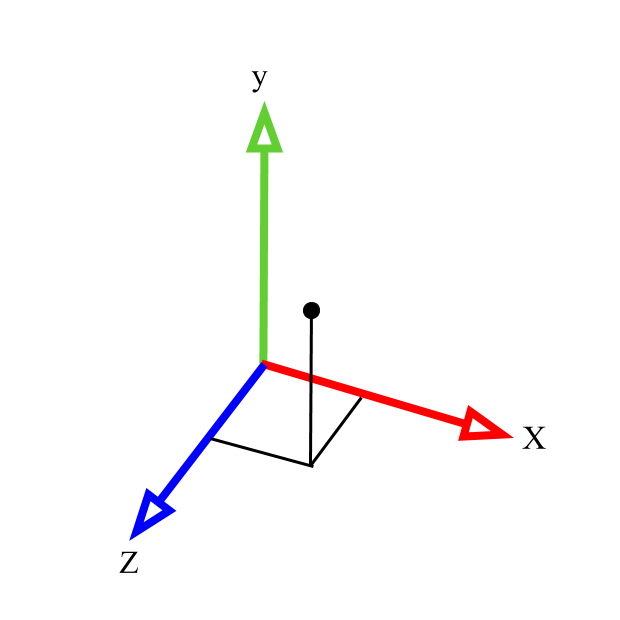
\includegraphics[scale=0.17]{Diagrams/3D_Axis.png}
		\caption{Point in 3D space shown using cartesian coordinates.}
		\label{3DAxisFigure}
	}
\end{figure}
\FloatBarrier

\begin{figure}[htbp]
	\raggedright
	{\centering
		\vspace{7px}
		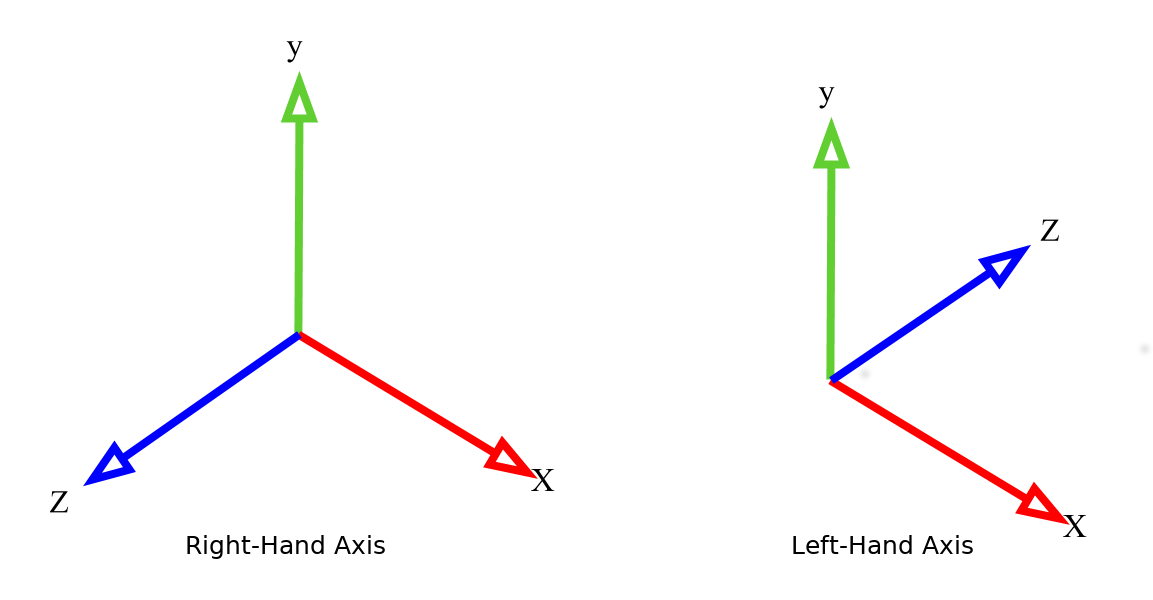
\includegraphics[scale=0.2]{Diagrams/HandAxis.png}
		\caption{Right Hand and Left Hand Coordinate Systems.}
		\label{3DAxisFigure}
	}
\end{figure}
\FloatBarrier

\subsection{Vector}


\section{Matrices}

\section{Quaternions}

